%% =====================================================================
%%  poglavlja/02_profiliranje_skupa.tex -- Analiza i profiliranje D-Fire
%% =====================================================================

\section{Analiza i profiliranje skupa podataka D-Fire}

\subsection{Naziv skupa podataka i izvor}
Odabrani skup podataka je \emph{D-Fire: an image dataset for fire and smoke detection}, koji objavljuje organizacija GAIA Solutions on Demand \cite{dfire}. Zvanični opis i poveznice za preuzimanje nalaze se u GitHub repozitoriju D-Fire \cite{dfire}. Repozitorij uglavnom sadrži dokumentaciju i pomoćne datoteke, dok se sam skup slika i njihovih anotacija preuzima putem zasebnih poveznica navedenih u \texttt{README.md} datoteci. Autori navode zasebne arhive sa slikama i oznakama, pripremljenim podjelama te poveznicu na Kaggle verziju \cite{kaggle}.

Podaci nisu organizovani kao jedna CSV tabela. Osnovni sadržaj su rasterske digitalne slike i odgovarajuće tekstualne anotacije u YOLO formatu (\texttt{.txt}). Slikovne datoteke u pregledanoj kopiji imaju nastavak \texttt{.jpg}. Provjereni su povezivanje slika s oznakama i raspodjela po podskupovima.

\subsection{Opis, svrha i domen primjene}
D-Fire je namijenjen razvoju algoritama računarskog vida za otkrivanje prisustva i lokacije vatre i dima. Primjena uključuje video-nadzor, monitoring prirodnih područja i pravovremeno upozoravanje na potencijalni požar. Za razliku od obične klasifikacije cijele slike, detekcija objekata određuje i gdje se na slici nalazi traženi objekat. Skup obuhvata pojedinačne slike koje potiču iz nadzornih kamera, s interneta i iz javnih skupova podataka \cite{dfire}. Analizirana lokalna kopija sadrži slikovne datoteke i pripadajuće tekstualne anotacije; ne sadrži videodatoteke. Različiti izvori slika podrazumijevaju raznovrsne prikaze scena, udaljenosti objekata i uslove fotografisanja.

\subsection{Struktura skupa podataka}

\subsubsection{Slike, klase i anotacije}
Anotacije su namijenjene detekciji dvije klase objekata:
\begin{itemize}
  \item dim (\emph{smoke});
  \item vatra (\emph{fire}).
\end{itemize}
Slike se, za potrebe opisne statistike, mogu grupisati u četiri međusobno isključive kategorije slika: samo vatra, samo dim, i vatra i dim, niti vatra niti dim. Ovo nisu četiri klase objekata u YOLO modelu. Jedna slika može sadržavati više objekata i više pravougaonih anotacija.

Kod uobičajene YOLO tekstualne oznake svaki red predstavlja jedan objekat:
\begin{verbatim}
class_id x_center y_center width height
\end{verbatim}

\subsubsection{Organizacija foldera i podjela}
D-Fire nije organizovan tako da svaki folder predstavlja jednu klasu: objekti se mogu pojaviti zajedno, pa se klase čitaju iz anotacija. Pregledana lokalna kopija ima sljedeću strukturu:
\begin{verbatim}
D-Fire/
  train/
    images/  (17.221 slika)
    labels/  (17.221 oznaka)
  test/
    images/  (4.306 slika)
    labels/  (4.306 oznaka)
\end{verbatim}
Trening dio čini 80,00\%, a testni 20,00\% slika. Nema zasebnog validacijskog foldera. Validacijski dio za buduće treniranje treba izdvojiti iz trening skupa. Testni dio namijenjen je završnoj evaluaciji.

\subsection{Veličina skupa podataka}
Prema zvanično objavljenim brojkama, D-Fire sadrži ukupno 21.527 slika i 26.557 označenih objekata (\emph{bounding boxes}) \cite{dfire}. Lokalnim prebrojavanjem potvrđeni su isti brojevi (Tabela~\ref{tab:prof-kategorije} i Tabela~\ref{tab:prof-objekti}). Raspodjele su dobijene čitanjem izvornih oznaka.

\begin{table}[H]
\centering
\small
\begin{tabular}{@{}lrr@{}}
\toprule
\textbf{Kategorija slike} & \textbf{Broj slika} & \textbf{Udio}\\
\midrule
Samo vatra & 1.164 & 5,41\%\\
Samo dim & 5.867 & 27,25\%\\
Vatra i dim & 4.658 & 21,64\%\\
Bez vatre i dima & 9.838 & 45,70\%\\
\midrule
\textbf{Ukupno} & \textbf{21.527} & \textbf{100,00\%}\\
\bottomrule
\end{tabular}
\caption{Raspodjela slika po međusobno isključivim kategorijama.}
\label{tab:prof-kategorije}
\end{table}

\begin{table}[H]
\centering
\small
\begin{tabular}{@{}lrr@{}}
\toprule
\textbf{Klasa objekta} & \textbf{Bounding box oznaka} & \textbf{Udio}\\
\midrule
Vatra & 14.692 & 55,32\%\\
Dim & 11.865 & 44,68\%\\
\midrule
\textbf{Ukupno} & \textbf{26.557} & \textbf{100,00\%}\\
\bottomrule
\end{tabular}
\caption{Broj označenih objekata po klasi.}
\label{tab:prof-objekti}
\end{table}

U 5.822 slike prisutna je vatra (samostalno ili s dimom), a u 10.525 slika prisutan je dim (samostalno ili s vatrom). Ova dva broja se ne sabiraju u 21.527 jer se 4.658 slika pojavljuje u obje grupe. U skupu je ukupno 11.689 pozitivnih slika (najmanje jedan ciljani objekat) i 9.838 negativnih slika. Ovi brojevi potvrđeni su čitanjem lokalnih oznaka i odgovaraju zvaničnoj tabeli. Negativne slike imaju postojeću, praznu datoteku oznaka.

\subsection{Tipovi podataka i važnost karakteristika}
Skup sadrži slike u boji i tekstualne YOLO oznake. Oznake sadrže klasu objekta te numeričke podatke o njegovom položaju i veličini (Tabela~\ref{tab:prof-podskupovi} i Slika~\ref{fig:prof-raspodjela}).

\begin{table}[H]
\centering
\small
\begin{tabular}{@{}lrrr@{}}
\toprule
\textbf{Kategorija} & \textbf{Trening} & \textbf{Test} & \textbf{Ukupno}\\
\midrule
Samo vatra & 944 & 220 & 1.164\\
Samo dim & 4.681 & 1.186 & 5.867\\
Vatra i dim & 3.763 & 895 & 4.658\\
Bez vatre i dima & 7.833 & 2.005 & 9.838\\
\midrule
\textbf{Sve slike} & \textbf{17.221} & \textbf{4.306} & \textbf{21.527}\\
\bottomrule
\end{tabular}
\caption{Lokalno izmjerena raspodjela slika po podskupovima.}
\label{tab:prof-podskupovi}
\end{table}

\begin{figure}[H]
\centering
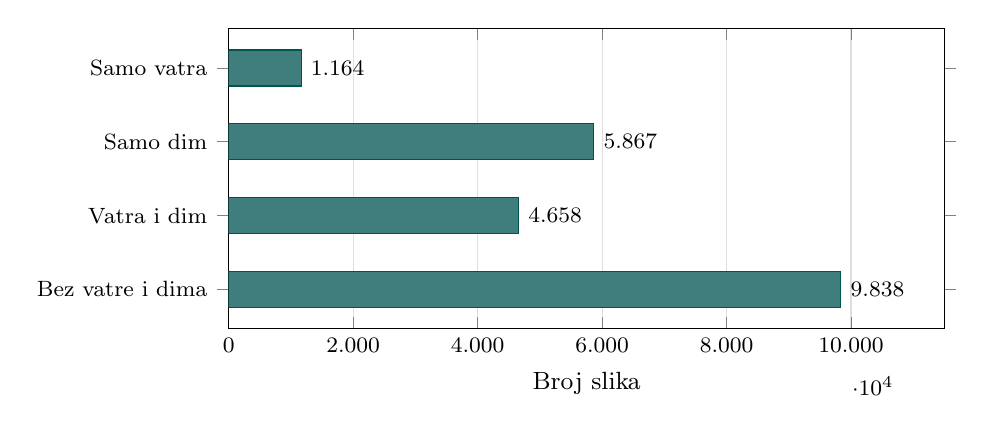
\begin{tikzpicture}
\begin{axis}[
  xbar, width=0.88\linewidth, height=5.4cm,
  symbolic y coords={Bez vatre i dima,Vatra i dim,Samo dim,Samo vatra},
  ytick=data, xmin=0, xmax=11500, bar width=13pt, enlarge y limits=0.18,
  xlabel={Broj slika},
  tick label style={font=\footnotesize}, label style={font=\small},
  xtick={0,2000,4000,6000,8000,10000},
  xticklabels={0,2.000,4.000,6.000,8.000,10.000},
  nodes near coords, nodes near coords align={horizontal},
  every node near coord/.append style={font=\footnotesize},
  /pgf/number format/.cd, fixed, use comma, 1000 sep={.},
  xmajorgrids=true, grid style={solid,gray!25}]
\addplot[fill=teal!65!black!75, draw=teal!65!black] coordinates {
  (9838,Bez vatre i dima)
  (4658,Vatra i dim)
  (5867,Samo dim)
  (1164,Samo vatra)
};
\end{axis}
\end{tikzpicture}
\caption{Raspodjela slika prema izvornim oznakama; lokalni rezultat odgovara \cite{dfire}.}
\label{fig:prof-raspodjela}
\end{figure}

\subsection{Raspodjela podataka i osnovne statistike}

\subsubsection{Zastupljenost kategorija}
Kategorije nemaju jednak broj slika: slika sa samo vatrom ima 1.164, a slika bez vatre i dima 9.838. Broj označenih objekata je ujednačeniji: 14.692 oznake vatre i 11.865 oznaka dima. Jedna slika može sadržavati više objekata, pa broj slika i broj objekata treba razlikovati. Pri treniranju treba obratiti pažnju na slabije zastupljene primjere i provjeriti koliko uspješno model prepoznaje i vatru i dim.

\subsubsection{Dimenzije slika i numeričke varijable}
Tabela~\ref{tab:prof-dimenzije} sadrži mjerenja nad svih 21.527 uspješno dekodiranih slika. Aritmetička sredina označena je kao prosjek, a omjer stranica računa se kao širina podijeljena visinom. Ekstremi širine i visine posmatraju se zasebno i ne moraju pripadati istoj slici.

\begin{table}[H]
\centering
\small
\begin{tabular}{@{}lrrrr@{}}
\toprule
\textbf{Mjera} & \textbf{Min.} & \textbf{Maks.} & \textbf{Prosjek} & \textbf{Medijana}\\
\midrule
Širina slike (px) & 162 & 4.288 & 984,27 & 1.061\\
Visina slike (px) & 142 & 2.848 & 582,10 & 700\\
Omjer širina/visina & 0,45 & 3,84 & 1,6880 & 1,7778\\
\bottomrule
\end{tabular}
\caption{Lokalno izmjerene dimenzije slika i omjer stranica.}
\label{tab:prof-dimenzije}
\end{table}

Prosječne dimenzije trening slika iznose $985,26\times 582,89$\,px, a testnih $980,32\times 578,92$\,px. Slični prosjeci ne dokazuju jednakost scena ili uslova snimanja. Raspon rezolucija pokazuje potrebu za ujednačavanjem ulaza modela; promjena veličine uz dopunjavanje rubova čuva omjer stranica i zahtijeva odgovarajuću transformaciju oznaka.

\subsection{Kvalitet i varijabilnost slika}

\subsubsection{Uslovi snimanja}
Raznovrsni izvori sugerišu promjenjive pozadine, uglove kamere, udaljenosti od požara, osvjetljenje, kontrast, boje i veličine ciljanih objekata. Na javno prikazanim primjerima uočavaju se i udaljeni pejzaži, gust dim i plamen različitog intenziteta \cite{dfire}. Takva raznolikost je korisna za generalizaciju, ali otežava razlikovanje dima od magle, oblaka i pare, a plamena od odsjaja i jarko osvijetljenih površina.

\subsubsection{Realne i sintetičke slike}
Skup uključuje slike stvarnih scena iz nadzornih kamera \cite{dfire}. Udio sintetičkih, renderovanih ili generisanih slika nije utvrđen jer takva podjela nije navedena u oznakama.

\subsubsection{Duplikati i granice provjere curenja podataka}
SHA-256 sažetak izračunat je nad cijelim sadržajem svake slike. Nije pronađena nijedna grupa identičnih datoteka, ni unutar podskupova ni između trening i testnog dijela. Taj rezultat ne isključuje iste slike u drugačijem kodiranju, susjedne video-kadrove ili isti prizor. Vizuelna sličnost, identitet kamere i semantička ispravnost oznaka nisu provjereni ovim automatskim profiliranjem.

\subsection{Razlog izbora skupa podataka}
D-Fire je prikladan za zadatak detekcije vatre i dima jer ima više od 21 hiljade slika, gotove prostorne anotacije, oba ciljana objekta i veliki broj negativnih primjera. Time omogućava treniranje i vrednovanje modela koji istovremeno prepoznaje klasu i locira objekat. Raznoliki izvori slika povećavaju relevantnost problema za praktične scenarije, uz potrebu pažljive kontrole kvaliteta i odvajanja podataka.

\subsection{Najbitnije karakteristike za detekciju}
Boja i nepravilni oblici plamena pomažu prepoznavanju vatre, dok je za dim važna njegova raspršena tekstura. Položaj i veličina označenih okvira omogućavaju modelu da nauči gdje se vatra i dim nalaze na slici.

\subsection{Zaključak}
D-Fire sadrži 21.527 slika namijenjenih detekciji vatre i dima, podijeljenih na 17.221 trening i 4.306 testnih slika. Analizom su prikazani raspodjela kategorija, broj označenih objekata i osnovne statistike dimenzija slika. Skup uključuje i slike bez vatre i dima, koje su važne za smanjenje lažnih alarma.

Kategorije nisu jednako zastupljene, a slike se razlikuju po rezoluciji i uslovima snimanja. To treba uzeti u obzir pri pripremi podataka i treniranju modela. Raznovrsnost primjera i gotove oznake čine ovaj skup prikladnom osnovom za daljnji rad na detekciji vatre i dima.